\documentclass[sigchi-a]{acmart}

\usepackage{booktabs} % For formal tables
\usepackage{framed}
\usepackage{color}
\usepackage{caption}
\usepackage[font=small]{subcaption}
\usepackage{multicol}

% Copyright
%\setcopyright{none}
%\setcopyright{acmcopyright}
%\setcopyright{acmlicensed}
%\setcopyright{rightsretained}
%\setcopyright{usgov}
%\setcopyright{usgovmixed}
%\setcopyright{cagov}
%\setcopyright{cagovmixed}
\copyrightyear{2018}
\acmYear{2018}
\setcopyright{rightsretained}
\acmConference[MOCO]{5th International Conference on Movement and
Computing}{June 28--30, 2018}{Genoa, Italy}
\acmBooktitle{MOCO: 5th International Conference on Movement and Computing, June
28--30, 2018, Genoa, Italy}\acmDOI{10.1145/3212721.3212882}
\acmISBN{978-1-4503-6504-8/18/06}


\newenvironment{Figure}
  {\par\medskip\noindent\minipage{\textwidth}}
  {\endminipage\par\medskip}

\begin{document}


\title{\emph{Improv}: Live Coding for Robot Motion Design}

\author{Alexandra Q. Nilles}
\affiliation{%
  \institution{Department of Computer Science \\ University of Illinois at Urbana-Champaign}
    }
\email{nilles2@illinois.edu}

\author{Chase Gladish}
\affiliation{%
  \institution{Department of Computer Science \\ University of Illinois at Urbana-Champaign}
    }
\email{gladish2@illinois.edu}

\author{Mattox Beckman}
\affiliation{%
  \institution{Department of Computer Science \\ University of Illinois at Urbana-Champaign}
    }
\email{mattox@illinois.edu}

\author{Amy LaViers}
\affiliation{%
  \institution{Mechanical Science and Engineering Department \\ University of Illinois at Urbana-Champaign}
    }
\email{alaviers@illinois.edu}


% The default list of authors is too long for headers.
\renewcommand{\shortauthors}{A. Nilles et al.}

 \begin{CCSXML}
<ccs2012>
<concept>
<concept_id>10010520.10010553.10010554.10010558</concept_id>
<concept_desc>Computer systems organization~External interfaces for
robotics</concept_desc>
<concept_significance>500</concept_significance>
</concept>
%<concept>
%<concept_id>10010405.10010469</concept_id>
%<concept_desc>Applied computing~Arts and humanities</concept_desc>
%<concept_significance>300</concept_significance>
%</concept>
</ccs2012>
\end{CCSXML}
%
\ccsdesc[500]{Computer systems organization~External interfaces for robotics}
%\ccsdesc[300]{Applied computing~Arts and humanities}

\begin{abstract}

Often, people such as educators, artists, and researchers wish to quickly
generate robot motion. However, current toolchains for programming robots can be difficult to
learn, especially for people without technical training.
This paper presents the \emph{Improv} system, a programming language for
high-level description of robot motion with immediate visualization of the
resulting motion on a physical or simulated robot. \emph{Improv} includes a 
"live coding" wrapper for ROS (``Robot Operating
System", an open-source robot software framework which is widely used in
academia and industry, and integrated with many commercially available robots).
Commands in \emph{Improv} are compiled to ROS
messages. The language is inspired by choreographic techniques, and allows the
user to compose and transform movements in space and time. In this
paper, we present our work on \emph{Improv} so far, as well as the design decisions made
throughout its creation.
\end{abstract}




%
% The code below should be generated by the tool at
% http://dl.acm.org/ccs.cfm
% Please copy and paste the code instead of the example below.
%

\keywords{robotics, choreography, live coding, ROS, Haskell, roshask,
human-robot interaction}

\maketitle

\begin{marginfigure}
\centering
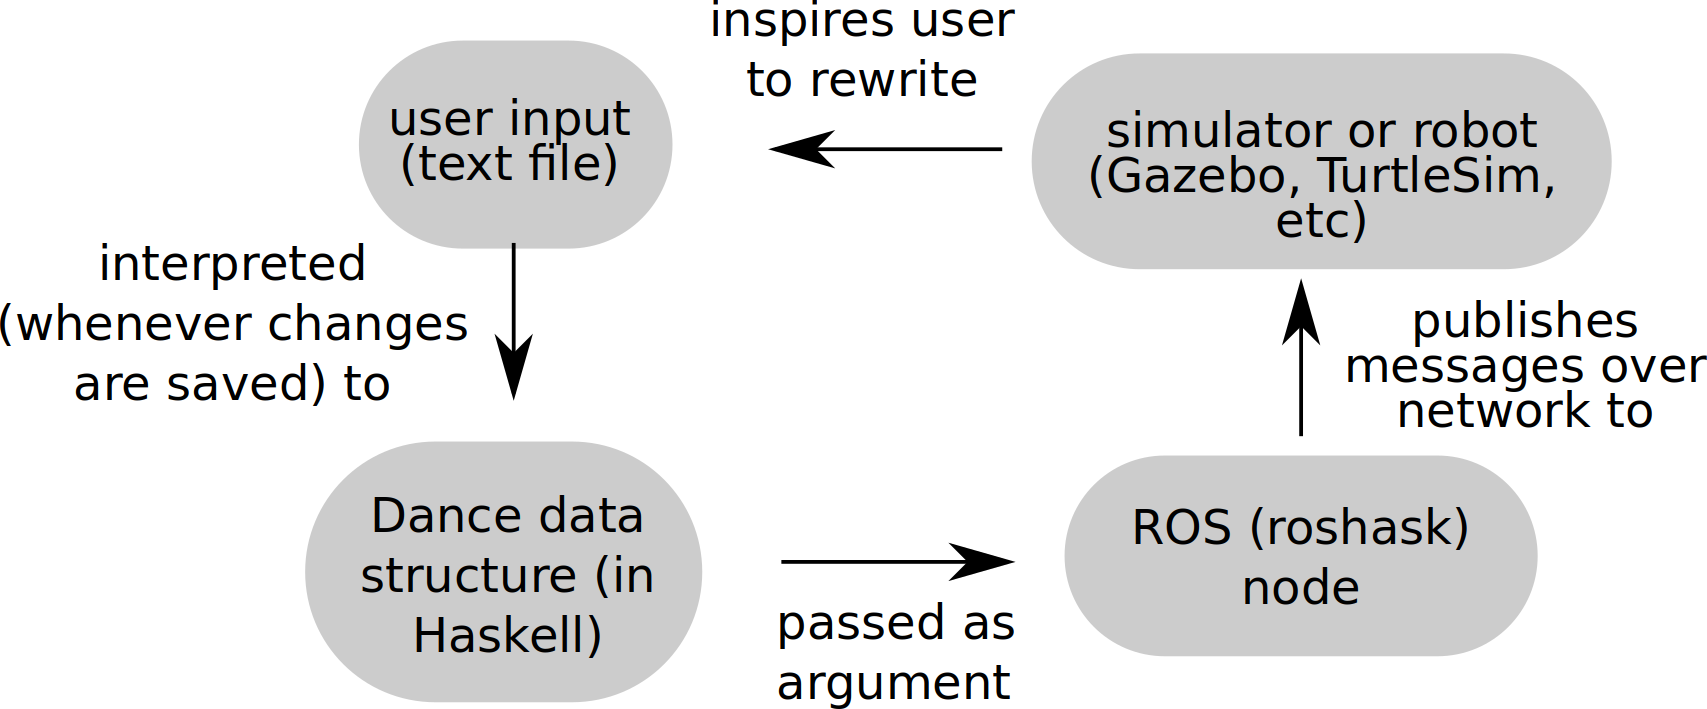
\includegraphics[width=\marginparwidth]{flowchart.png}
\caption{An illustration of how user input, written to a text file, is
converted into a ROS node which publishes messages to a simulator or physical 
robot.
\label{flowchart}}

\vspace{2em}
\end{marginfigure}



\section{Introduction}\label{introduction}

Robotic technology is becoming more commonly integrated into settings outside of
the factory - including classrooms \cite{mataric2004robotics} and art
installations \cite{kukaDance2017}. In many of these cases, users often do not
have extensive programming experience, and only require the robot to follow specific motion
patterns and perhaps have simple reactivity. The time is
ripe for \emph{choreographic} methods of programming robots, which
match our mental models of motion.

\begin{sidebar}
The following ROS Python client code will cause a
mobile robot such as a Roomba or Turtlebot to follow a path that curves
forward and left:
\end{sidebar}

\newcommand*{\MyIndent}{\hspace*{0.5cm}}

\begin{margintable}
\begin{tabular}{l}
\texttt{if \_\_name$\_\_ ==$ '\_\_main\_\_':} \\ 
\MyIndent \texttt{pub = rospy.Publisher(} \\
\MyIndent \MyIndent \texttt{'turtle1/cmd\_vel',Twist)} \\ 
\MyIndent \texttt{rospy.init\_node('publisher\_node')} \\ 
\MyIndent \texttt{loop\_rate = rospy.Rate(5)} \\ 
\MyIndent \texttt{while not rospy.is\_shutdown():} \\ 
\MyIndent \MyIndent        \texttt{vel=Twist()} \\
\MyIndent \MyIndent        \texttt{vel.linear.x = 1.0} \\
\MyIndent \MyIndent        \texttt{vel.angular.z = 1.0} \\
\MyIndent \MyIndent        \texttt{pub.publish(vel)} \\
\MyIndent \MyIndent        \texttt{loop\_rate.sleep()}
\end{tabular}
\end{margintable}

\begin{sidebar}
The equivalent code in \emph{Improv} is

\vspace{1em}

\texttt{
turtle1 \$ forward || left
}

\vspace{1em}

where $||$ is an operator which combines movements in parallel.
\end{sidebar}

Currently, many commercially available robots are programmed through interfaces
(which may be graphical, text-based, or physically interactive)
created for each specific robot by the manufacturer or through ROS (the "Robot Operating
System") \cite{rossano2013easy} \cite{quigley2009ros}. We target an improved user experience for ROS, because it is a
free and open source toolset which is compatible with many platforms. \emph{Improv} is essentially a wrapper around ROS. This gives us the
benefits of ROS's infrastructure, but we exchange the powerful low-level control
available in most ROS client libraries for the simplicity of a high-level
representation of robot motion.

The ROS workflow has two obstacles for newcomers to robotics programming: 1)
programs are written at a low level of abstraction, requiring users to
painstakingly translate their mental model of the intended movement, and 2) the
process of writing code, compiling and executing the instructions on the robot
platform can be intimidating. For example, a beginner
tutorial for ROS will have the user open at least three terminal windows, a text
editor, and a robot simulator, for a total of five windows. It is often not
possible to see all the relevant windows at one time, making it difficult for the user to have a coherent mental model of
information flow in the system.

The tool introduced in this paper, \emph{Improv}, addresses both of these
sticking points. With \emph{Improv} we hope to help make robotics more accessible to a broader
range of people. Possible users of this tool include artists, educators,
newcomers to robotics, and anyone who wishes to quickly prototype robot motion
patterns. \emph{Improv} is open-source and available at
\url{https://github.com/alexandroid000/improv}. Please let us know if you try it
out!


\subsubsection*{Related Work}

\begin{sidebar}

\subsection{Live coding and algorave}

This work is heavily influenced by live coding interfaces and programming
languages for generating music and visuals, which are often associated with the
algorave performance movement \cite{collins2014algorave}. In particular, the
programming language TidalCycles \cite{mclean2010tidal} has had a strong
influence on the structure of the \emph{Improv} programming language, both 
syntactically and in how relative timing of events is managed. Also worth
mentioning is \emph{Al Jazari}, a live coding installation which uses a simple
graphical language to allow people to control robots (in simulation)
\cite{mclean2010visualisation}. The language includes conditionals based on
external state and communication between the bots. The program state of the
robot is also visualized. There are a variety of other projects centered around
live coding interfaces for controlling cyberphysical systems and visual
simulators \cite{livecoding14}.

\vspace{1em}

One important design decision for developers of interactive text-based
programming tools is whether to tie their tool to a specific text editor. 
 We decided to allow
users flexibility to choose their editor of preference.
Instead of creating an interface for each desired
editor, we use a shell script which monitors the file that the user is
editing for changes. Every time the user saves changes to the file, the
program detects a change, interprets the user's new program, and restarts the ROS node. This design choice circumvents the need to
interface with specific editors. While we have not done a formal timing
analysis, the delay is a small fraction of a second and not noticeably longer than the
time it takes to look from the text editor to the simulator.

\end{sidebar}

Especially when used with the two-dimensional Turtlesim, \emph{Improv}
is reminiscent of \emph{Logo} \cite{logo}, an educational language that is often used in conjunction with a simulation of a
two-dimensional turtle. Our programming language is less expressive and powerful 
than \emph{Logo}, but is integrated with ROS and thus able to be used with
three-dimensional simulators and actual robots. Scratch, an educational, visual
programming language has been integrated
with ROS \cite{crick2017rosbridge}, which is the most closely
related work to \emph{Improv}. Our interface is textual, while Scratch is
visual, and the \emph{Improv} programming language is more focused on modelling 
of choreographic concepts (such as relative timings of movements and body
symmetries) while Scratch is focused on game development.

Among many programming languages for robotics \cite{nordmann2016survey}, we are aware of two other tools for live
programming in ROS, one which uses the Python shell \cite{python_live_DSLRob}, and one
which uses the Live Robot Programming language and the Pharo ROS client 
\cite{campusano2017live} \cite{estefo2014towards}.
However, these languages focus on low-level sensor and
actuator commands and logical control flow, rather than modeling movement. 
These tools are better suited for
applications which involve sensing the environment, while
\emph{Improv} is better suited to applications where the user wishes to quickly
generate certain movements and creatively explore movement patterns.
\emph{Improv} is heavily influenced by \emph{Dance}, a
domain-specific language inspired by Labanotation and built in Haskell \cite{Dance2003}. Another relevant project is
\emph{roshask} \cite{cowley2011stream}, a Haskell client library for ROS, which
this project uses as an interface between our domain-specific language and ROS.

%\subsubsection*{Paper Outline}
%
%Section \ref{embodied} details how this work was inspired by embodied
%improvisation for robot motion design, as well as concepts from the field of human-computer
%interaction, and the resulting design principles for the tool.
%Section
%\ref{architecture-overview} provides an overview of the software architecture,
%how the features of \emph{Improv} implement
%our design principles, and some example programs. Section
%\ref{domain-specific-language-design} describes some of the design decisions and
%features of the high-level domain-specific language, as well as the
%corresponding design choices in the Haskell backend. 
%Section \ref{interfacing-with-ros} details more about how ROS messages are
%defined for specific robotic platforms, and how the live coding interface is
%implemented. Finally, Section
%\ref{conclusions-and-future-work} summarizes our conclusions and outlines directions
%for future work, including user studies.
%


%\begin{figure*}
% \centering
%\includegraphics[width=0.9\textwidth]{/home/alli/common/figs/rosfig.jpg}
%\captionof{figure}{An example of a typical workflow in ROS, created by following a
%beginner tutorial. There are five overlapping terminal windows open, as well
%as the Gazebo simulator. \label{rosfig}}
%\end{figure*}

\section{Prototyping Movement Design in Embodied Improvisation}\label{embodied}


\emph{Improv} is a tool for \emph{prototyping} robot motion. Put another way, it
is a tool for improvising movement on robot platforms. The authors have taken
inspiration from their experiences with embodied improvisation, and the
creative movement design it enables. Movement experts have analyzed strategies for
improvisation for choreography and performance \cite{forsythe2004improvisation}.
Improvisation helps the movement designer understand and explore the plethora of
movement options that are available at any given time. This is especially useful
in robotics applications as the field starts to explore stylized movement and
the incorporation of robotic technology into homes and art installations. 

However, the time taken to set up environments and write, compile and
execute code often negates the benefits of improvisational practice when done
on a robotic platform instead of a human body. These barriers especially
affect those users who do not have a strong background in programming. This places
some design constraints on the \emph{Improv} system - namely, the system must
have


\begin{itemize}
\item a minimal ``representational
distance" between the user's mental model of the movement and
its description in code, so there is minimal frustration and time wasted in
translation,
\item a near-imperceptible delay between writing instructions to the robot and
seeing the effect of those instructions, and
\item a singular environment where the
user interacts with the program (to avoid the user's attentional flow being
broken by needing to switch between different interaction modalities).
\end{itemize}


\section{\emph{Improv} Features}\label{architecture-overview}
\begin{sidebar}
The authors were influenced by several of the principles
outlined in the `cognitive dimensions of notations' \cite{green1996usability}.
There are eleven `cognitive dimensions,' or design principles, that the authors
describe but several are especially relevant to this work, such as

\begin{itemize}
\item \emph{Closeness of mapping}: "Ideally, the
problem entities in the user's task domain could be mapped directly onto
task-specific program entities, and operations on those problem entities would
likewise be mapped directly onto program operations" \cite{green1996usability}
\item \emph{Diffuseness}: How many symbols or graphic entities are required to express a meaning?
\item \emph{Error-proneness}: Does the design of the notation induce `careless mistakes'?
\item \emph{Hard mental operations}: Are there places where the user needs to resort to  fingers or pencilled annotation to keep track of what's happening?
\item \emph{Progressive evaluation}: Can a partially-complete program be executed to
obtain feedback on `How am I doing'?
\end{itemize}

%The \emph{Improv} language addresses the cognitive
%dimensions \emph{closeness of mapping} and \emph{diffuseness}: as the example in the introduction showed, we
%are able to express a movement such as ``curve forward and left" very concisely. The user is also not required to translate their
%concept of ``curve forward and to the left" to low-level instructions such as the 
%rotational velocities of the robot's wheels.
%
%Less noisy code also
%helps with \emph{error-proneness}, since the user does not need to manually
%configure as many settings. We have also tried to make our parser flexible, by
%allowing different amounts of whitespace between lines and operators, though
%this area could certainly use more improvement. The final two features, the fast
%compile time and simple user environment, both help reduce \emph{hard mental
%operations} and gives the user a fast and easy way to use \emph{progressive
%evaluation}.
\end{sidebar}

To specifically address these design criteria, we have
included the following features in \emph{Improv}.
These features are intended to give the user a sense of \emph{flow}: a
mental state of complete absorption in the activity. The fewer distractions in the activity, whether it is improvisational dance or coding,
the higher the chance of the participant becoming completely engaged and
accessing all the available creative options.

\begin{itemize}
\item \emph{small representational distance between
movement and code:} a domain-specific language, inspired by choreographic
techniques such as spatial symmetries, relative timing changes, and body-centric
coordinates. The systems and terminology developed by choreographers and other movement
experts are invaluable in this attempt, such as in \cite{laviers2017choreographic} \cite{cuykendall2014designing} \cite{alaoui2014choreography} and
\cite{humphrey1959art}.
\item \emph{rapid movement prototyping:} changes to the user's file are interpreted by a 
Haskell program that builds a ROS node for publishing messages to a
simulator or physical robot. This process is nearly real time, allowing for a
seamless user experience.


\item \emph{workspace with few attentional switches:}
a live coding interface with only two windows at most, one for editing the text file and
one for observing effects on a simulated robot.
%Currently, we have tested the
%system with:
%\begin{itemize}
%  \item
%    TurtleSim: a two dimensional simulator where
%    velocity commands nearly perfectly control an animated turtle.
%  \item
%    Gazebo with a TurtleBot robot model: a three-dimensional simulator
%    with more realistic physics, where velocity commands control
%    simulated motors.
%  \end{itemize}
\end{itemize}


%As examples of possible user interfaces, Figure \ref{guiex} shows an example of 
%the system in use. Note that the choice of
%editor and the choice of simulator are decoupled, and \emph{Improv} is
%absolutely editor-agnostic, relying only on an operating-system level script
%to execute changes. \emph{Improv} is somewhat simulator-agnostic: 
%currently it is only possible to control robots which use a \texttt{Twist} ROS messages
%for control, which set desired linear and rotational
%velocities.

\subsubsection{Domain Specific Language (DSL) Features}\label{domain-specific-language-design}


The base type of the \emph{Improv} language is a movement. Movements can be combined with each other in various ways, forming new
movements. Table \ref{grammar} shows the grammar of the \emph{Improv} language.
The language supports primitive robot movements such as \texttt{forward} and \texttt{right}. 
Movements are organized in units of time called 
``beats.'' The base timing of beats (units per minute) can be specified by the
user. Movements can be composed and stored in variables. The following table shows some
example programs in \emph{Improv}.


\begin{tabular}{p{0.25\linewidth} p{0.3\linewidth} p{0.35\linewidth}}

\hline

Natural Language & Code & Comments \\

\hline

\emph{move forward for one beat, turn right for one beat, move forward for one beat}  & \texttt{forward right forward} & performed in three beats \\

\hline

\emph{move forward, right, and forward, all in one beat} & \texttt{[forward right forward]} &
performed in one beat - same spatial extent, but faster \\

\hline

\emph{curve right and forward} & \texttt{forward \textbar{}\textbar{} right} & \\

\hline

%\emph{move forward four times} & \texttt{repeat 4 forward} & \\


%\emph{do movement \texttt{x}, reflected across saggital plane} & \texttt{reflect YZ x} & \\
%
%\hline

\emph{reverse the movement "forward right left"} & \texttt{reverse (forward right left)} & same as \texttt{left\ right\ forward} - reverses the order of the primitives \\
%
\hline

\emph{retrograde the movement "forward right left"} & \texttt{retrograde (forward right left)} & same as \texttt{right\ left\ backward} - reverses entire trajectory \\

\end{tabular}



%While we have only implemented these combinators for simple and very
%symmetric mobile robots, one could imagine making more complicated types
%of symmetry for other robot platforms. We have included a typeclass
%\texttt{Symmetric\ a}, parameterized by a body type \texttt{a}, and defined by a function
%\texttt{refl\ ::\ Plane\ -\textgreater{}\ a\ -\textgreater{}\ a}. By defining this
%typeclass once for a new robot platform, detailing all the different symmetries of
%the body, the functionality of these spatial transformers can be
%extended to new platforms.

%\subsection{Multiple Robots}\label{multiple-robots}
%
%The \emph{Improv} system has the capability to control multiple robots
%at once, using a syntax which mirrors how \emph{TidalCycles} allows for
%multiple tracks to be played simultaneously. Each robot is given a
%unique name in the shell script which launches ROS and the \emph{Improv}
%system (this is also where the initial location of each robot is
%specified). Then, in the user's program, they specify which movement
%sequence should be associated with each robot. For example, to make
%robot \texttt{r1} move forward and robot \texttt{r2} move backward, the
%user would write
%
%\begin{verbatim}
%r1 $ forward
%r2 $ backward
%\end{verbatim}
%
%This syntax, along with assigning movements to variables, can make it easy to
%specify relationships between how different robots are moving, such as
%
%\begin{verbatim}
%x = left right [forward right]
%r1 $ x
%r2 $ retrograde x
%\end{verbatim}
%
%
%which would cause robot \texttt{r2} to perform the same movement as
%robot \texttt{r1}, but in retrograde. It is also possible to command two robots
%to do the same movement with a program such as
%
%\begin{verbatim}
%r1 r2 $ forward backward
%\end{verbatim}
%
%As \emph{Improv} is extended to other platforms in the future, this could be an
%interesting mechanism for studying how the same high-level choreographic
%commands are perceived when executed on different platforms.

% \subsection{Modelling Movement in
% Haskell}\label{modelling-movement-in-haskell}

%Programs in the \emph{Improv} DSL are interpreted by a compiled Haskell
%program into an abstract data type (ADT), which represents each
%\texttt{movement}. This ADT, which we call a \texttt{Dance}, can be thought of as
%a tree that holds all movement primitives and their compositions and
%transformations. To
%execute a \texttt{Dance} as a series of ROS messages, we must flatten
%the tree while maintaining their relative timing information, which will
%be discussed in Section \ref{relative-timing}.
%
%\texttt{Dance}s are defined as
%
%\begin{verbatim}
%data Dance b = Prim Action Mult b
%             | Rest Mult
%             | Skip
%             | Dance b :+: Dance b
%             | Dance b :||: Dance b
%\end{verbatim}
%
%where \texttt{Prim} is a motion primitive type, composed of the
%\texttt{Action} (direction and spatial extent of the movement),
%\texttt{Mult} which stores timing information, and \texttt{b}, a parameterized type describing the
%part of the robot to move. \texttt{Rest} indicates that the robot part
%is not moving for some period of time (and is a primitive in the
%\emph{Improv} language). 
%
%\texttt{Skip} is the identity dance, having no
%effect on the robot for no time duration, and is necessary for the
%monoidal structure of the parallel and
%series operators (\texttt{:\textbar{}\textbar{}:} and \texttt{:+:},
%respectively), which are binary operators on \texttt{Dance}s.
%
%This algebraic structure helps enforce the timing behavior that we
%expect; namely, associativity. If \texttt{d1}, \texttt{d2}, and
%\texttt{d3} are all \texttt{Dance}s (with an arbitrary number and
%structure of movement primitives in each), then we want to ensure the
%following equivalence:
%
%\begin{verbatim}
%(d1 :+: d2) :+: d3 = d1 :+: (d2 :+: d3).
%\end{verbatim}

%{\color{red} clean up - what are two/three most important features of haskell
%that help?}
%
%Similarly, if three \texttt{Dance}s are in parallel, arbitrary groupings
%should not change the meaning of the program. This is exactly the
%behavior that the algebraic objects \emph{monoids} have: 
%associativity and an identity element. See \cite{yorgey2012monoids} for a much more
%detailed discussion on the usefulness of monoids in modelling and
%programming languages, in the context of \emph{Diagrams}, a Haskell DSL
%for creating vector graphics.
%
%We create monoid instances in Haskell for these operators on
%\texttt{Dance} data types, which allow for lists of \texttt{Dance}s to be combined
%in sequence or parallel. This is useful because the parser returns expressions
%in the user's program as a list of \texttt{Dance}s. By implementing our intuitive understanding that movements in parallel and
%series should be associative as an algebraic structure, we can use the power of Haskell's abstractions to
%get the correct behavior ``for free."
%
%Similarly, we use the Haskell functionality for mapping functions over data structures
%(such as our \texttt{Dance} trees) to implement transformers such as
%\texttt{retrograde} and \texttt{reverse}. We define these functions recursively
%over the \texttt{Dance} ADT, by first defining a function \texttt{transform}
%which has two arguments: the first, a function transforming individual
%\texttt{Action}s (for example, flipping them over a spatial axis, or shrinking
%their extent), and the
%second being a \texttt{Dance}. The \texttt{transform} function then returns the
%transformed \texttt{Dance}. This allows us to abstract out transformations from the
%low-level details of how they are propagated through the ADT, making it easier
%to implement new transformers.

%\subsection{Relative Timing}\label{relative-timing}
%
%As programs are parsed and converted to ROS messages, we must enforce the timing semantics - for example, movements
%inside square brackets, such as \texttt{{[}forward\ right\ forward{]}},
%must occur within one ``beat.'' The parser returns such a program as a list of \texttt{Dance}s, labelled with a type
%that indicates that they should be compressed in sequence.
%Then we call a function \texttt{seqL} which uses the length of the
% list to determine how much to speed up each individual dance
%before composing the movements. This is accomplished with a function
%\texttt{changeTiming} which takes a multiplier \texttt{m} and a
%\texttt{Dance}, and propagates the multiplier through the \texttt{Dance}
%recursively. This allows for nested sequential movements: for example,
%the program \texttt{{[}forward\ {[}left\ left{]}\ forward{]}} would
%result in timing multipliers \texttt{[3, 6, 6, 3]}. Note that the \texttt{left}
%primitives will have \texttt{Mult}s of 6, since
%they must occur six times as fast as normal to allow the whole movement
%to occur in one ``beat.'' Thus, movements are able to be arbitrarily sped up by
%placing them in sequence inside square brackets. Movements can only be slowed
%down by decreasing the \texttt{beat} parameter in the program file, which sets
%the number of time units per minute. By making this number smaller, movements
%such as a quarter turn will be slowed down to fill the specified unit of time.
%Future work may include a language primitive which is able to do this for
%smaller chunks of code inside the program file, instead of needing to change the
%global timing parameter.




\section{Conclusions and Future
Work}\label{conclusions-and-future-work}

\begin{margintable}
\begin{tabular}{rl}
prim $\rightarrow$ & rest  \\
     $|$ & forward \\
     $|$ & left  \\
     $|$ & halfleft\\
     $|$ & right \\
     $|$ & halfright \\
\\
movement $\rightarrow$ & prim \\
         $|$ & movement movement \\
         $|$ & [movement] \\
         $|$ & (movement) \\
         $|$ & movement $||$ movement  \\
         $|$ & transformer movement \\
\\
transformer $\rightarrow$ & reverse \\
  $|$ & retrograde \\
  $|$ & repeat n \\
  $|$ & reflect ax \\
\\
exp $\rightarrow$ & rs \$ movement \\
    $|$ & var $=$ movement
\end{tabular}

\caption{The grammar of \emph{Improv} programs. \texttt{exp} represents top-level
expressions, which execute movements on robot(s), or store movements in
variables. Movements are converted into ROS message streams and can be
composed and grouped in multiple ways. \label{grammar}}
\end{margintable}

% \begin{sidebar}
% 
% \section{Interfacing with ROS}\label{interfacing-with-ros}
% 
% \emph{Roshask} is a client library for ROS, written in Haskell. Features of this
% language allow for movement commands to be combined and transformed in more
% natural ways than imperative ROS client libraries. Haskell also is well-suited
% for building new programming languages.
% 
% The primitives in \emph{Improv}, such as \texttt{forward} or \texttt{right}, are
% mapped to ROS messages. In our implementation so far, we have mapped
% to the \texttt{Twist} ROS message, which specifies the robot's linear and
% angular velocity as two three-dimensional vectors. Velocity controllers, which
% often are included with commercial robots, are required to create the low-level
% motor controls for reaching and maintaining the desired velocities. 

%To integrate a robot with \emph{Improv}, one must
%specify how to convert the \texttt{Dance} data structure to a list of ROS
%messages. For example, for a non-articulated symmetric mobile robot (such as a Roomba or
%TurtleBot), this is accomplished by two functions: \texttt{moveBase} and
%\texttt{danceToMsg}. Since the robot has only one body part, \texttt{moveBase}
%takes an \texttt{Action} (direction and extent of movement) and converts it to a
%single ROS velocity command (which sets the desired linear and rotational
%velocity in the plane). 
%Here, we have simplified the language
%by varying only three velocity values, the robot's \(x,y-\)velocity in
%the plane and its angular velocity in the plane.
%
%Since our discretization of movements is relational (for
%example, you can have \texttt{Full}, \texttt{Half}, and \texttt{Quarter} extent,
%and directions are related through symmetries), only a small number of these
%translations from \texttt{Action}s to velocities need to be explicitly defined
%and the rest can be derived through their relations. For example,
%\texttt{moveBase (A dir Half)} is defined as \texttt{fmap (*2) (moveBase (A dir
%Quarter))},
%where \texttt{fmap} maps the function \texttt{*2} over the values in the velocity
%command returned by \texttt{moveBase (A dir Quarter)}. This encodes the relationship
%that a \texttt{Half} extent is twice as far as a \texttt{Quarter}, thus the
%robot must move twice as fast in the same direction to travel twice the distance
%in the same amount of time. Defining these relationships explicitly helps speed
%up recalibration or extension of the platform to new robots and simulators -
%onwith mappings from \texttt{Dance}s to ROS messages need to be hard coded,
%and the rest are derived from the relations.
%
%Once this conversion (from a \texttt{Dance} data structure to a list of ROS messages)
%has been completed, the list of ROS messages is passed to a ROS
%node defined in \emph{roshask}. This node publishes the commands over the ROS network.
%Even if multiple robots are controlled, the system still only uses one ROS node
%which publishes to multiple topics. Work is ongoing on whether to extend the
%system to control multiple ROS nodes, and if so, how best to implement this
%feature.

%\end{sidebar}

Future work must include systematic studies of the usability of the
system, as compared to other tools such as Scratch and Python or C++ ROS
clients. From our own explorations of the tool, we have found that the
experience is quite engaging, especially when using a three-dimensional
physical simulator. We have included a video as supplemental information of
\emph{Improv} being used with Gazebo.


One major limitation of \emph{Improv} is that the language does not allow the
user to incorporate sensor
feedback. An interesting future
extension of this work would be to interface the
\emph{Improv} DSL with ROS subscribers and include the ability to react to sensor readings and environment state.
Another limitation of \emph{Improv} is the complexity of incorporating new robot platforms. Currently it is only possible to control 
simple, Roomba-like robots by setting linear and rotational
velocities.
Extending \emph{Improv} to more articulated robots requires defining the
conversion from \emph{Improv} programs to ROS messages in Haskell, and may be
especially tedious for robots with many body parts and degrees of freedom.
Future work will involve using ongoing work in the RAD Lab on compactly
describing patterns of robot body organization to make
this extension process more accessible.




%Many features and limitations of ROS are being improved with the ROS2
%project\footnote{\url{https://github.com/ros2/ros2/wiki}},
%However, as far as we are aware, there
%is no Haskell client library for ROS2. As the ROS2 project is developed, the
%\emph{Improv} project could be adapted to the new framework to increase its
%robustness and cross-platform functionality.

Finally, we would like to emphasize that the design decisions for how
\emph{Improv} programs are realized on robot platforms are relatively arbitrary
and a single robot could have a multitude of different implementations. As
Thecla Schiphorst has written, ``it is not technological constraints that hold
us back from using technology in new ways; technology changes at a tremendous
rate. Our willingness to explore beyond the constraints of our imagination has
the greatest effect'' \cite{schiphorst}. We hope that the implementation
described here opens up new avenues of imagination for how robot programming can
become more easily integrated into different forms of human movement expression.

\section{Acknowledgements}


This work is partially funded by NSF grant \#1328018 and DARPA grant \#D16AP00001.


\bibliographystyle{ACM-Reference-Format}
\bibliography{refs}

\begin{marginfigure}
    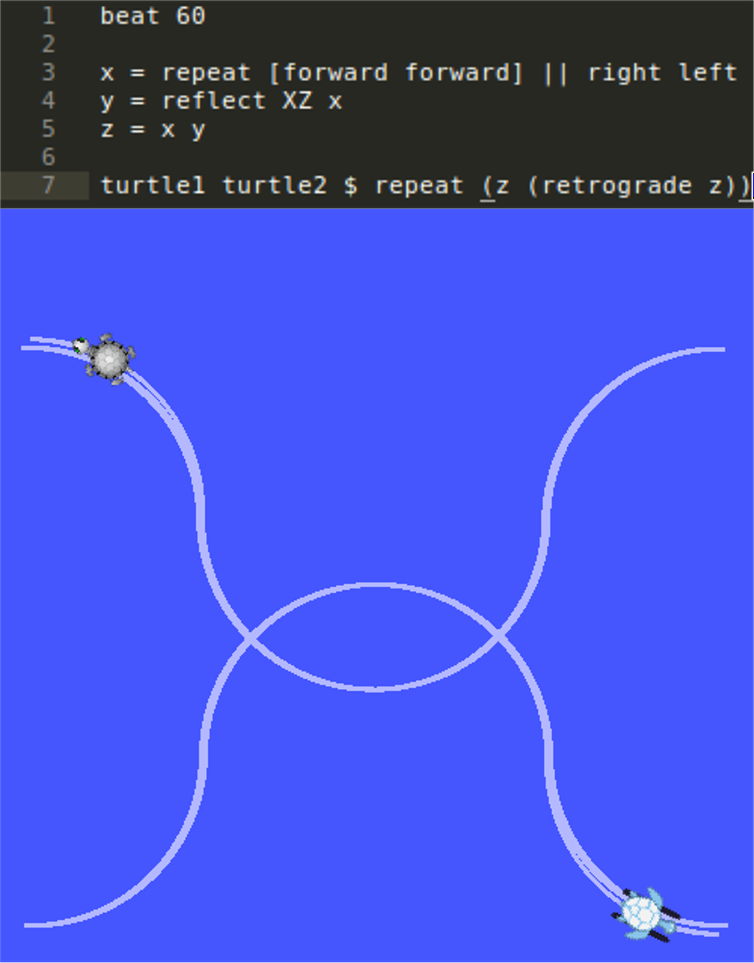
\includegraphics[width=\marginparwidth]{termturtle.png}
    %\captionof{figure}{A program as it appears in vim, a terminal-based text editor, with the
    % resulting movement in TurtleSim on two
    %simulated turtles.\label{vim}}
    \caption{An example of a text-editor and simulation environment
configuration available to users of \emph{Improv}. Any text editor can be
used, while simulators or robots must be compatible with the ROS message types
implemented with the system. \label{guiex}}
\end{marginfigure}

\end{document}
